\section{Usability Testing} \label{sec:usabilitytesting}
% Har svært ved hvornår jeg skal bruge usability testing eller usability test. Så det retter I bare til 

To gain a better understanding and detecting what issues could possibly arise when Ipsen interacts with the application, usability tests were conducted during the project. 
Usability testing results in possible usability issues which are guidelines to further improve the system's design. 

\subsection{Usability test setup and structure}
Before usability testing is conducted it is important to find out the purpose and objectives of the test. 
A task list will be defined based on the objectives of the usability test that the test subject need to complete using the application. The observations of the test consists of a test monitor, a screen video recording including audio and a video recording of the view of the PC screen and the test subject's interaction with the keyboard and the mouse. 
During the usability testing the test subject was asked to think aloud while performing a task to easily identify and categorize possible issues in \textit{critical}, \textit{serious} and \textit{cosmetic} which are described below \citep[p.~154]{brugervenligtwebdesign}.

\begin{itemize}
  \item Critical: An issue is classified as critical if the test subject are unable to continue and stopped completing tasks.
Critical issues can also involving high irritation while interacting with the application or if the test subject misunderstood one or more significant points of the application.
  \item Serious: If the test subject is significantly slowed down to completing tasks. 
This means the test subject has to use several minutes on a task.
	\item Cosmetic: When the test subject spends few minutes to completing a task and the issue is still should be solved. 
\end{itemize}

After a usability testing is conducted a debriefing session immediately  begins. 
Under debriefing session post-test questions will be asked for gain a deeper understanding of test subject's experience with the application overall. 
Here test subject is able to mention criticism of the interaction design and suggests solutions and design ideas. 
Besides a debriefing session's time frame should also allow for discussion if needed. 

Evaluation of the test will proceed as follows; while performing the usability testing the test monitor is taking notes of the possible issues and difficulties that test subject seems to encountered during interacting with the application. 
To better identify and categorize issues a screen recording with audio is reviewed and to ensure there is no missing observations.

\subsection{First usability test}\label{firsttest}
Based on the first interview with Ipsen a prototype for administrator role was created to generate a basic interface design from the requested requirements. 
This high-fidelity prototype consisted mostly of HTML and CSS code with focus on the design without implementation of the functionalities, see \Cref{sec:1prototype}.

\subsubsection*{Purpose and objectives of the first test}
This usability test's type was an exploratory test with purpose to represent the rough idea of how work flow of the different use cases could be operated in application. 
Ipsen would be represented for the interfaces where she would be able to navigate through the application.
This would provide Ipsen an overview of how the potential layout design might work with the functionalities that later would be implemented. 
The uncertain functionalities that might be useful for Ipsen will also be clarified during walk through of the prototype.
The test subject would be tested for these use cases below.

\begin{itemize}
	\item Add new file to the system
%represent the idea of how the add new document page interface could look like.
	\item Approval new version or document
%represent the idea of how approval process will work in the application.
	\item Access archive
%represent the idea of how the previous versions are stored in the Archive page and how to find them.
	\item Add user
	\item Manage user
%represent the idea of possible user administration interfaces. 
	\item Manage departments
%represent the idea of how the departments could be implemented. 	
\end{itemize}

\subsubsection*{Result of the first test}
Ipsen's reaction was mostly positive. 
She validated the idea of how the department management would be implemented. 
Ipsen also liked the overview of the user that both show those who are and those who are not associated to a specific department.
This would be useful if Ipsen possibly forgot to add some users to a department. 
The same applied to edit associated documents to the department page. 

Upload new version page and its main idea was that Ipsen would be able to marked version as a minor change or major change to notify readers. 
If the change is minor then readers could wait to read the new version.
And if it is a major change they need to read it now. 
Ipsen invalidate this functionality since the reader should not relate it and there is no need for that. 
The readers had typically have slightly reading skill. 
Therefore Ipsen prefer that it should be simple. 

Ipsen was satisfied with how accessing the archive work and manage user that was simple and straightforward. 

Ipsen thinked that it would be helpful to be able to search for a word in the documents.
For instance if a job title had change then she could search which document mention the job title that need to be modified.
This search functionality wished Ipsen only on the active documents. 

Whether the application is on English or Danish is unimportant. 
The application would therefore on English. 

Ipsen was overall satisfied with the prototype except the upload new version page that need to be redesign. 
Afterwards the prototype worked as a starting point for implementation of the application. 

\subsection{Second usability test}\label{secondtest}
This section will describe the second usability test	of type assessment test which was conducted on Ipsen and its results.

\subsubsection*{Purpose and objectives of the second test}
The majority requested functionalities for administrator role was implemented in the application at this point. 
Therefore the first usability test will only tested the administrator role part of the application.
The interaction between the test subject and the application must be validated to determine usefulness of the implemented functionalities. 
The purpose of the test is to identify general issues concerning the perception of the handbook application for further improvements of the application design.
The research questions, the method description and the task list can be found in \Cref{sec:utest2tasklist}.
The use cases below will be tested.

\begin{itemize}
	\item Access current handbook 
	\item Add new file to the system
	\item Approve new version or document
	\item Access archive 
	\item Add user 
	\item Manage departments
\end{itemize}

The functions of the system that will be tested are listed below.

\begin{itemize}
	\item Add document
	\item Add version
	\item Approve version
	\item Request approval
	\item Add user
	\item Add department
	\item Add user to department
	\item Add document to department
\end{itemize}

\subsubsection*{Results}
The identified issues discovered during the usability test will be presented and categorized below in \Cref{tab:utest2} with explainations following. 

\begin{table}[H]
	\begin{center}
	\begin{tabular}{| c | m{21em} | c | c | c | c | c |}
		\hline
		\# & \textbf{Identified usability issues} & Critical  & Serious & Cosmetic \\
		\hline
		 1 & Confusion regarding add and upload a new document   & x &  &  \\
		\hline
		 2 & No overview of existing document ID when creating a new document &  & x & \\
		\hline
		 3 & Confusion when creating a new version to a document & x & &  \\
		\hline
		4 & No indication when a version is sent to approval & x & & \\
		\hline
		5 & No indication on which page is currently showing &  &  & x \\
		\hline
		6 & Negative document ID &  & x & \\
		\hline
		7 & Not able to correct/modify a document ID & & x &  \\
		\hline
		8 & Department's associated users only presents as email &  &  & x \\
		\hline
	\end{tabular}
	\end{center}
	\caption{Identified issues for the second usability test}\label{tab:utest2}
\end{table}

The identified issue '1' occurred when Ipsen tried to create a new document and add a version to the document. 
As Ipsen thought that it is possible to both add a document and upload at the same time. 
The application at the current state would work such that user need to add a document first by enter the document name, chapter ID and section ID. 

Afterwards the user needed to find the document in the handbook and upload a new version. 
This created confusion which cause an interrupted work flow with the handbook.

The identified issue '2' took place when Ipsen attempted to create a new document. 
Ipsen needed to go back to the handbook's overview to check the existing document ID to be able find out which chapter the new document should belong to. 

The identified issue '3' occurred when Ipsen tried to create a new version to an existing document. 
It was unclear where to upload a new version. 
Therefore Ipsen tried to add a new document and then uploaded a new version. 
The upload button was not noticeable and took time before Ipsen found it. 

The identified issue '4' turned up as Ipsen tried to send a version to approval and then  approve the version herself.
Ipsen did not detect when she had sent the version to approval or whether she just approved the version. 
An indication or a message displayed to the user after a version is sent to approval or that the version is now approved and now are available in the handbook should solve this issue.

As identified issue '5' point out the confusion that occurred while Ipsen attempted to approve a version could be that the sidebar did not indicate which page she was currently on. 

The identified issues '6' and '7' appeared when Ipsen made a mistake as the application allowed her to enter a negative chapter and section ID. 
Ipsen felt the need to correct the mistake which the application did not support at the moment.
Ipsen wished to be able to delete a document that do not contain a version yet if a mistake occur.

The identified issue '8' occurred as Ipsen assigned a user to a department and noticed that users was presented as email address.
Ipsen preferred name instead of email address.

In the debriefing session Ipsen mentioned that she was surprised that the application required user to attached a pdf file as she has seen other document version control system has their own file editor.
However, Ipsen could see the reason behind it and commented that it is a good approach.
%Anna: Evt. kommenter at hun i virkeligheden selv havde sagt dette ikke skulle være en del af systemet til at starte med (evt henvis til iteration 1)

Ipsen also remarked that the features' names were clear and understandable. 

During the test session it had been clarified that administrator must be able to use the administrator right to get an awaiting approval approved without the other approvers had been through it.
The situations where other approvers either do not get it done, are too slow or are on a vacation could occur. 
The administrator right will therefore prevent possible bottleneck in the work flow.
%%% Andre kommentarer %%%
%Afdelingsleder holder styr på hvem der har læst hvad
%Kom frem til at admin skal kunne bruge sin admin ret til at få det godkendt hvis andre som blev sat til approvals ikke få det gjort (Kunne måske være relevant at kommenterer da det var noget vi tog til efterretning til næste test ) 
%Det virker ulogisk for pia i starten at den gældende version også i arkiver og ikke kun under handbook. Men synes til sidst at det smart når man skal audit og så det er nemt at finde frem (Anna: Tror jeg i stedet tager denne ned i iterationsafsnittet i stedet for hvis det er ok )

%en version er kun uploadet -- kan man slet den 
%en version som er blevet godkendt -- arkveret 

%Admin har en overrolloing hvis folk ikke går ind og godkender. Hvis folk tager for lang tid om det eller hvis folk er på ferie. (Anna: Samme kommentar som du har i starten af de her kommentarer )

\subsection{Third usability test}\label{thirdtest}
The third usability test was conducted on Ipsen right after the second test had finished. 

\subsubsection*{Purpose and objectives of the third test}
The tests that was conducted before had only focus on the administrator role.
The purpose of this third test was to validate the idea of how the interfaces for a writer and reader role could possibly look like. 
The mockups that was represented can be found in  %\Cref{} husk at tilføj det til bilag også. eller skal jeg bare tilføje dem her under ?

\subsubsection*{Results of the third test}
The major difference of the interface between administrator role from writer and reader role was the sidebar on the left, see \Cref{fig:mockupSidebar}.
Since writer and reader would not be able to access the most of the functionalities available on the sidebar.
The sidebar would therefore only appear for administrator. 
Ipsen agreed on the idea to keep the interface as simple as possible for both writers and readers. 

\begin{figure}[H]
	\centering
	\begin{subfigure}[b]{0.48\textwidth}
		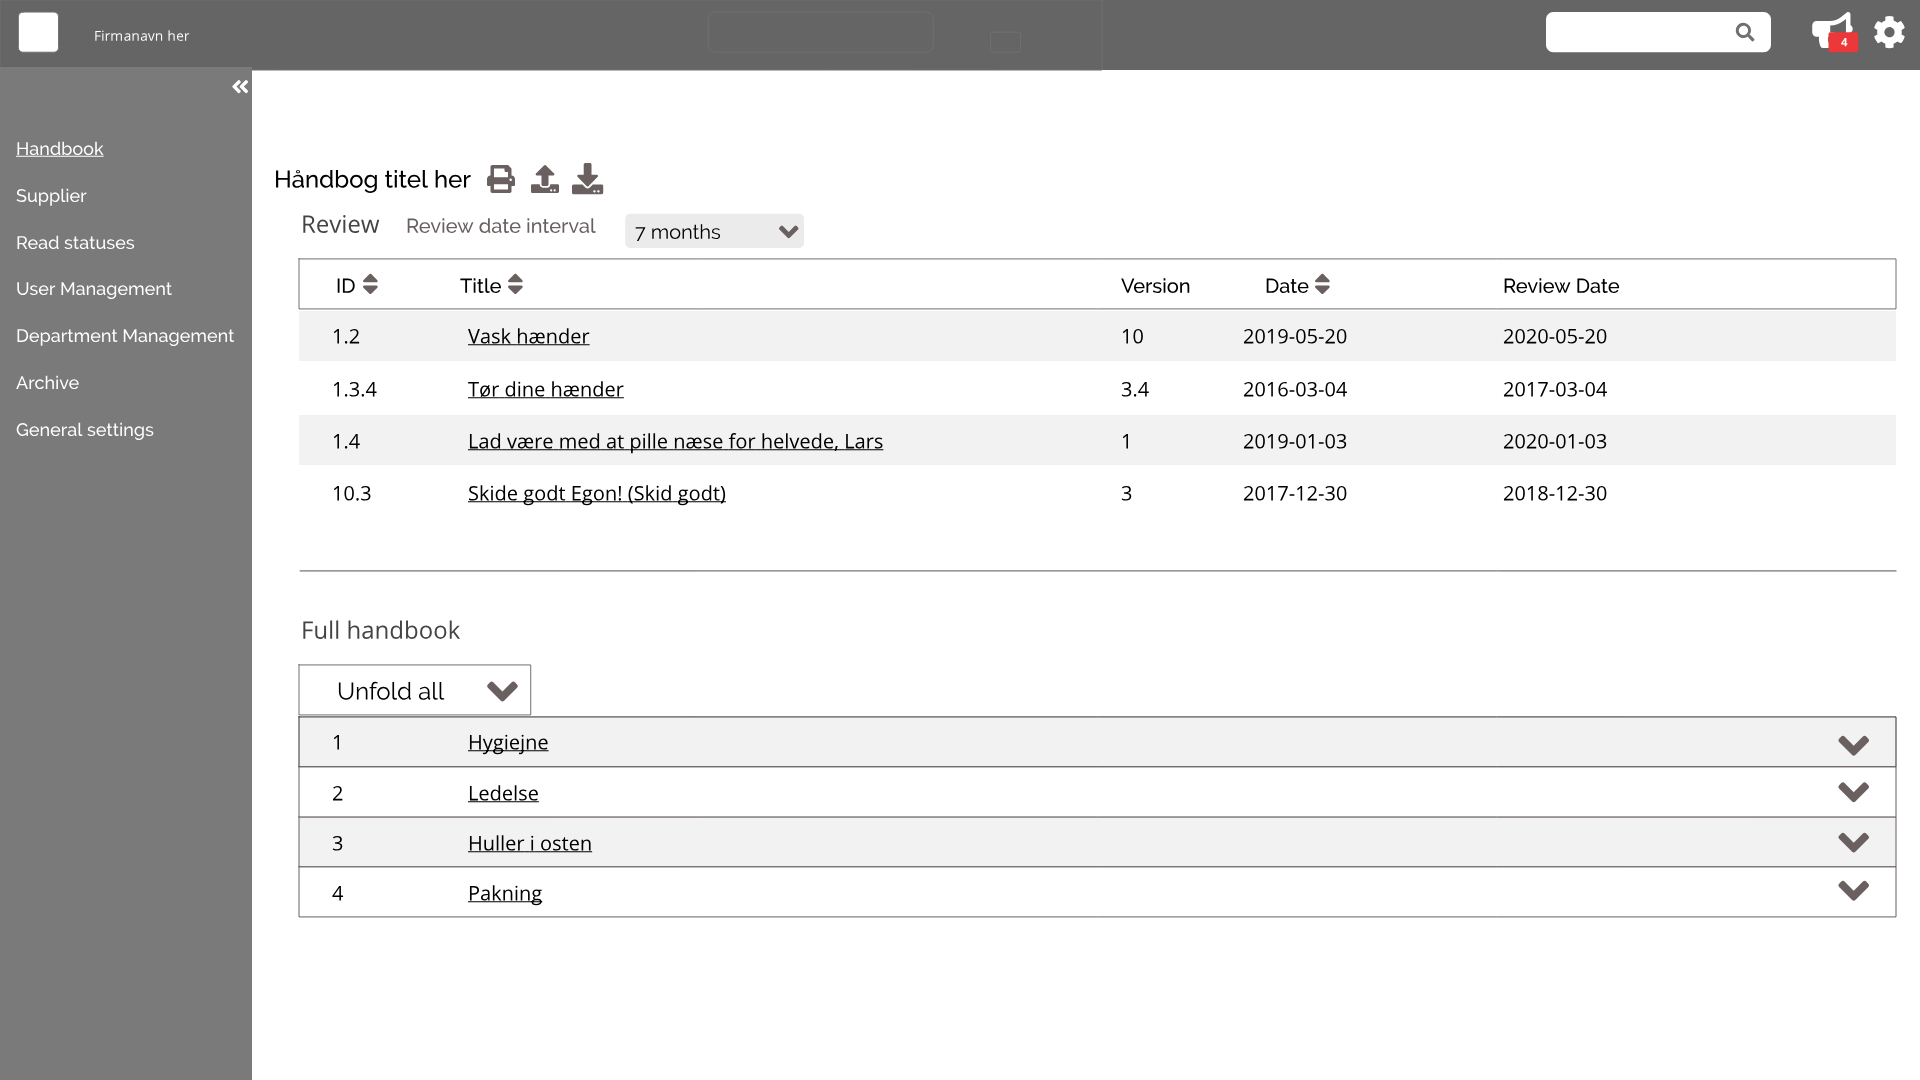
\includegraphics[width=\textwidth]{billeder/ForsideAdmin.jpg}
		\caption{Mockup interface for administrator}
		%\label{fig:3-main}
	\end{subfigure}
	\quad
	\begin{subfigure}[b]{0.48\textwidth}
		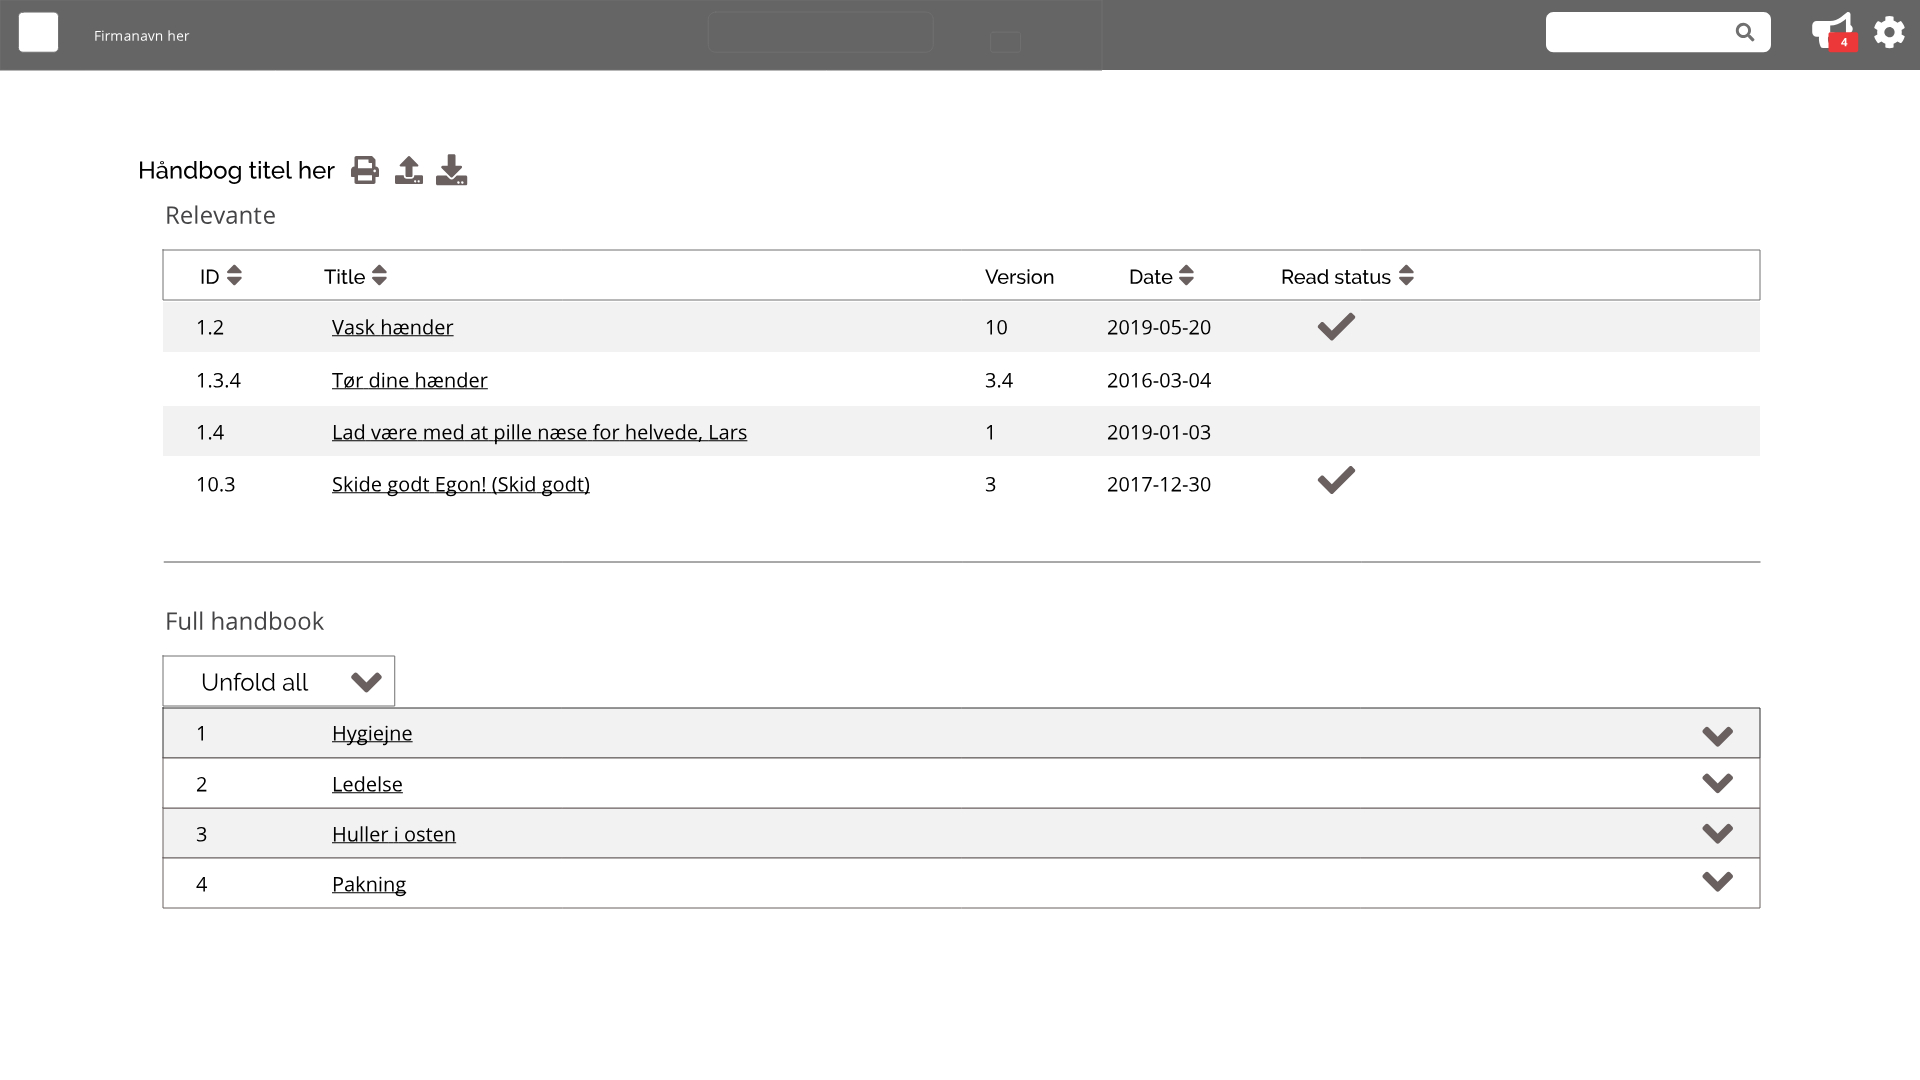
\includegraphics[width=\textwidth]{billeder/ForsideWriterReader.jpg}
		\caption{Mockup interface for writer and reader}
		%\label{fig:3-addDoc}
	\end{subfigure}
	\caption{Mockup interfaces comparision}\label{fig:mockupSidebar}
\end{figure}

In the mockup the handbook page consisted of division of relevant document that would be showed first on the top and the full handbook underneath.
For the reader role the relevant document would consist of those associated documents of the department they belonged to. 
And for the writer role the documents he had been assigned to approve would appear under the relevant document. 
Those document should be easy to find as well provide an overview and Ipsen validated the concept.

The idea of implementing a preview when user clicked on the document name was also showed to Ipsen. 
The user would have an opportunity to see a preview of a document before chosen to display it full screen, see \Cref{fig:mockupPreview}
This enable the user to better navigate through and still have an overview of the handbook which Ipsen also agreed upon.

\begin{figure}[H]
	\centering
	\begin{subfigure}[b]{0.48\textwidth}
		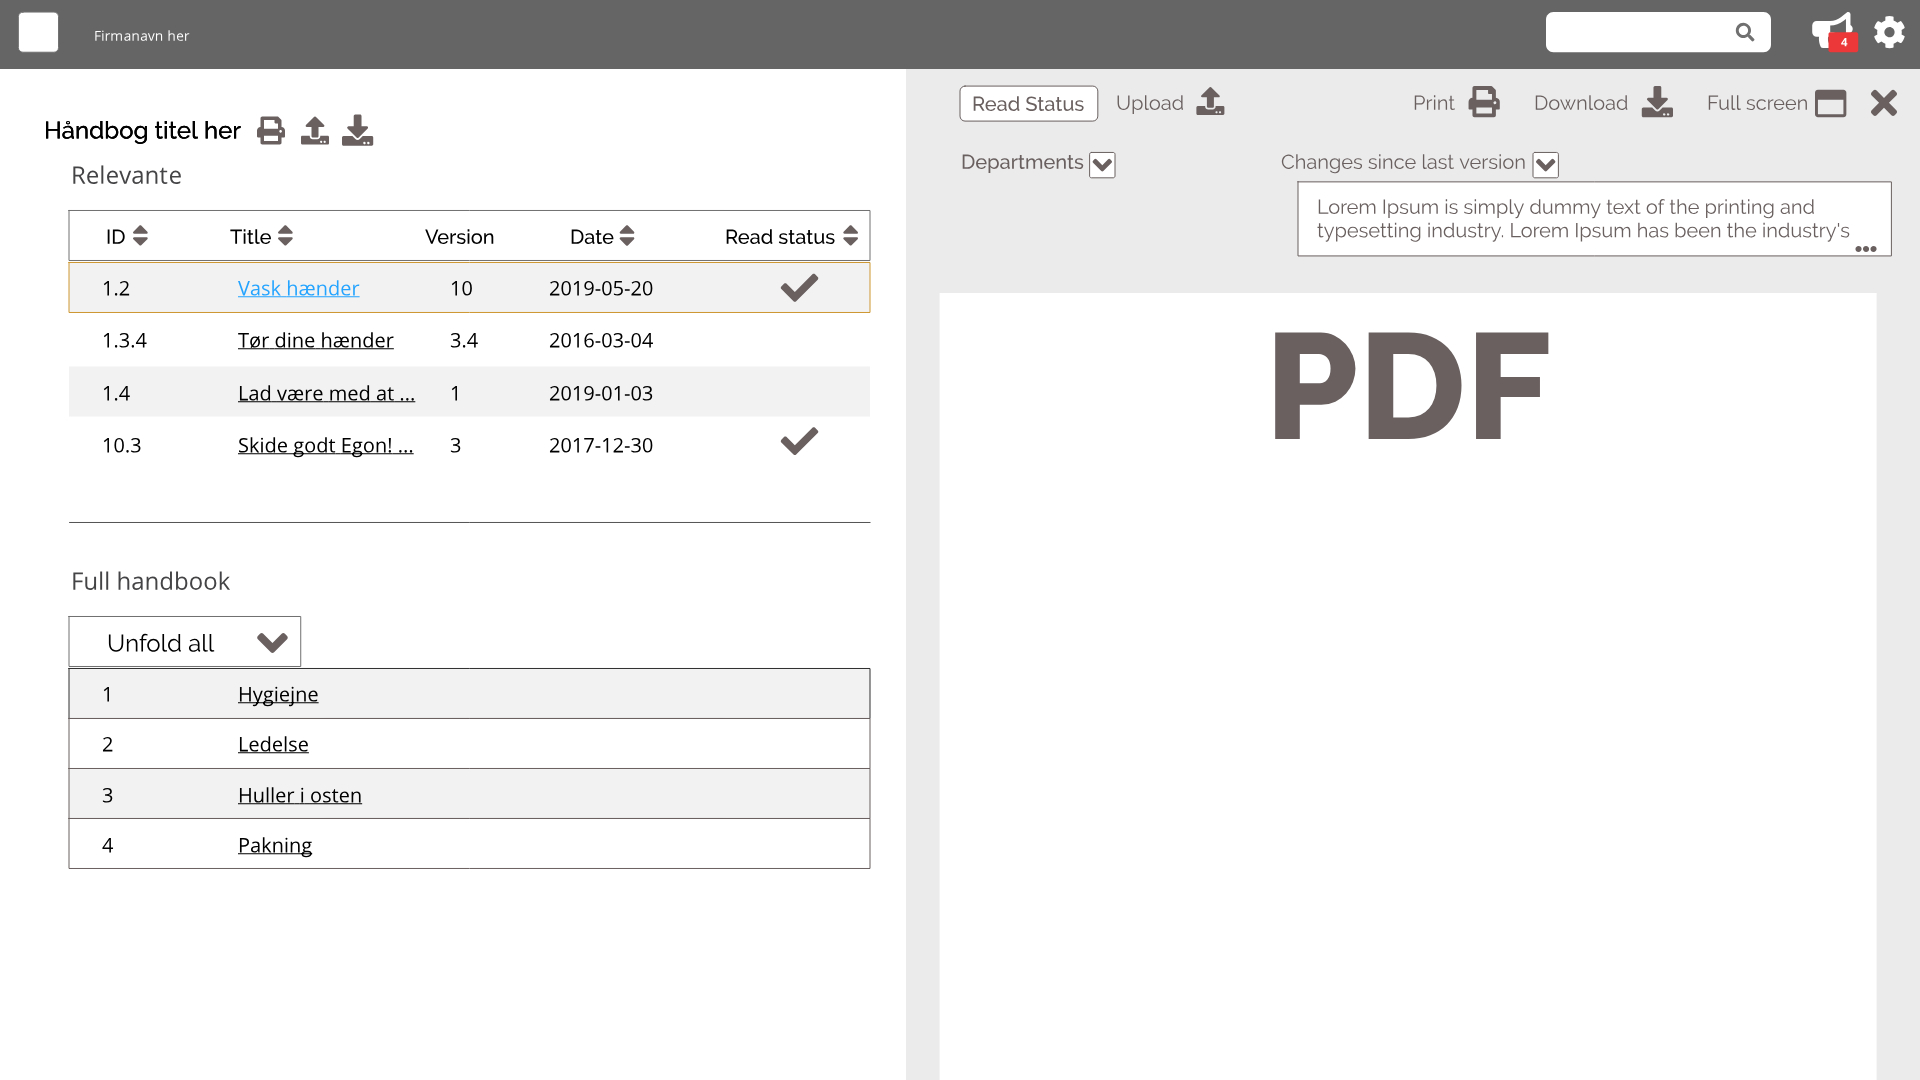
\includegraphics[width=\textwidth]{billeder/PreviewVersion.jpg}
		\caption{Mockup interface of document preview}
		%\label{fig:3-main}
	\end{subfigure}
	\quad
	\begin{subfigure}[b]{0.48\textwidth}
		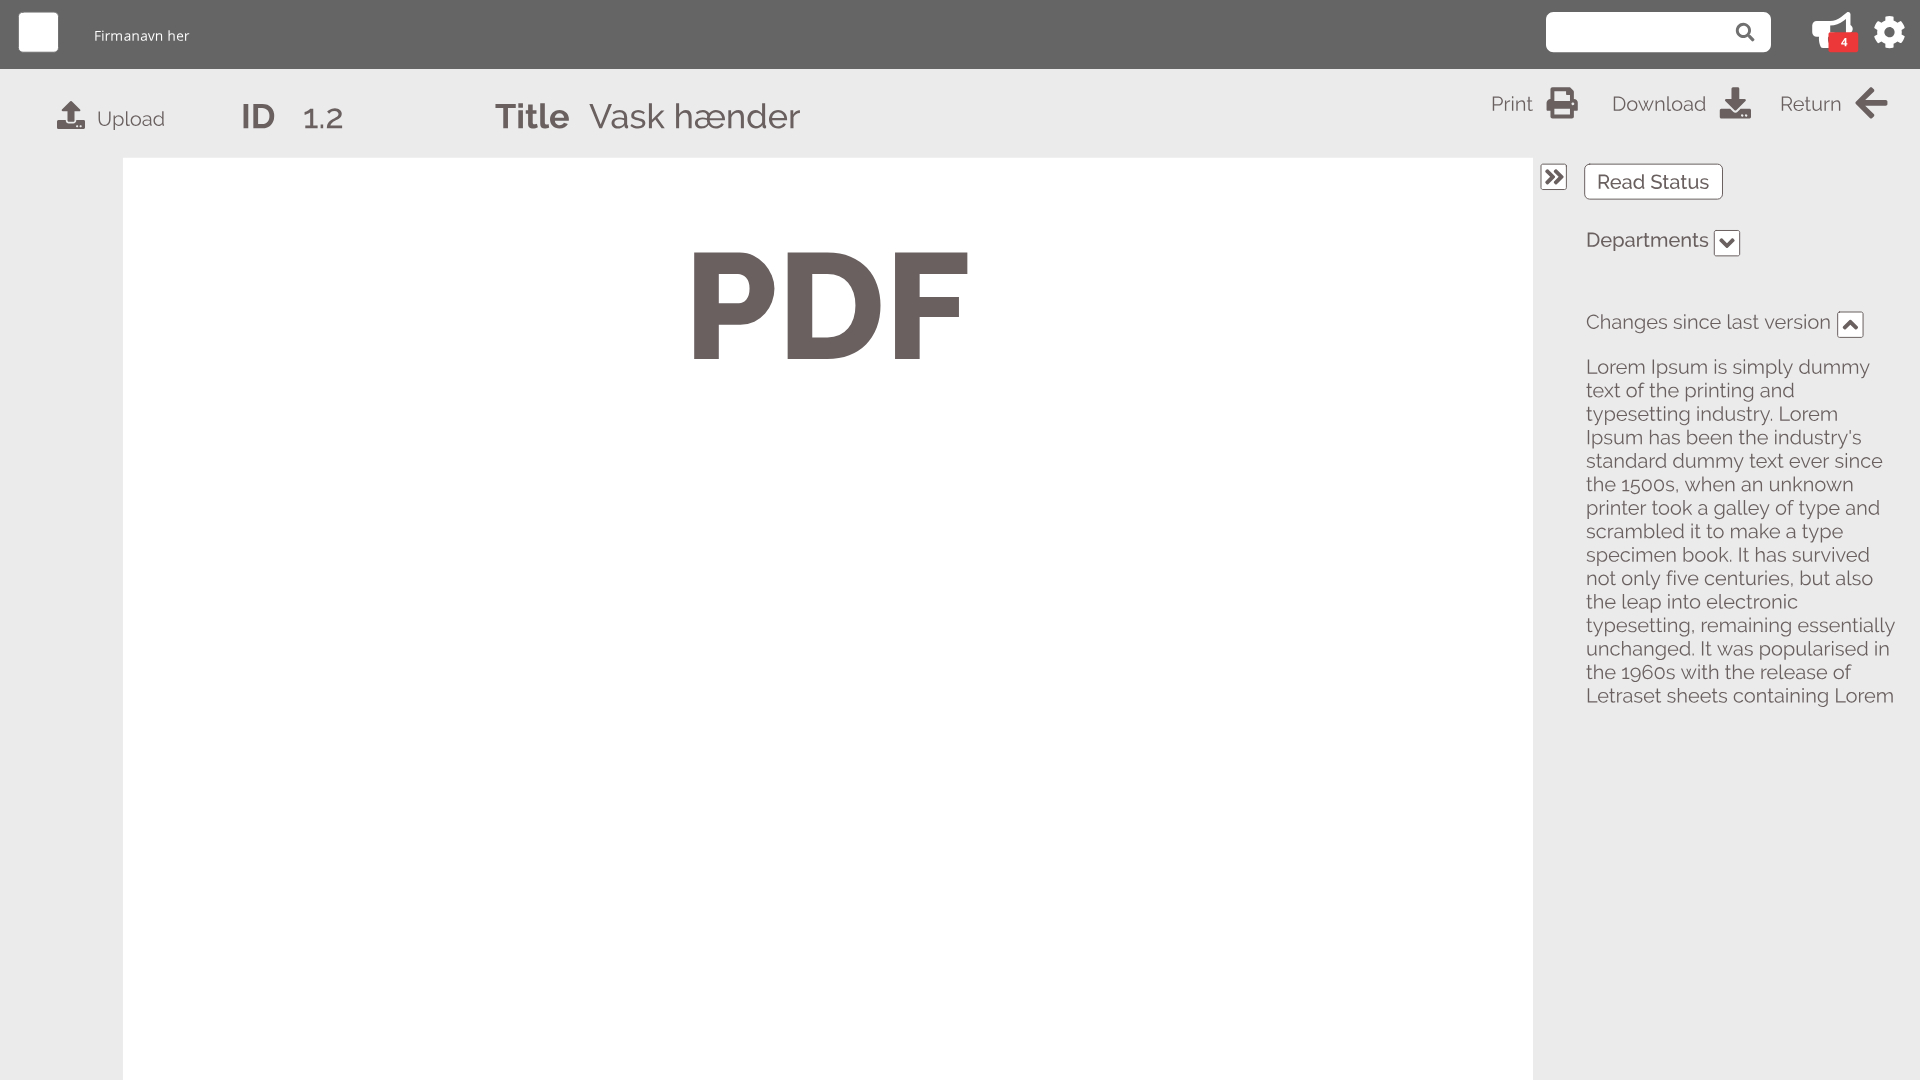
\includegraphics[width=\textwidth]{billeder/FullView.jpg}
		\caption{Mockup interface of document full view}
		%\label{fig:3-addDoc}
	\end{subfigure}
	\caption{Mockup interfaces of document preview and full view}\label{fig:mockupPreview}
\end{figure}

An interface change of the sidebar was also represented which applied to every role.
Beforehand the sidebar only contained informative text which the mockup now had added suitable icons as well. 
The user had two options with the sidebar.
Either could the sidebar be folded to only consist of icons, see \Cref{fig:mockupSidebarIcon} or unfold to see both the icons and informative text. 
Ipsen validated the new sidebar design. 

\begin{figure}[H]
	\centering
		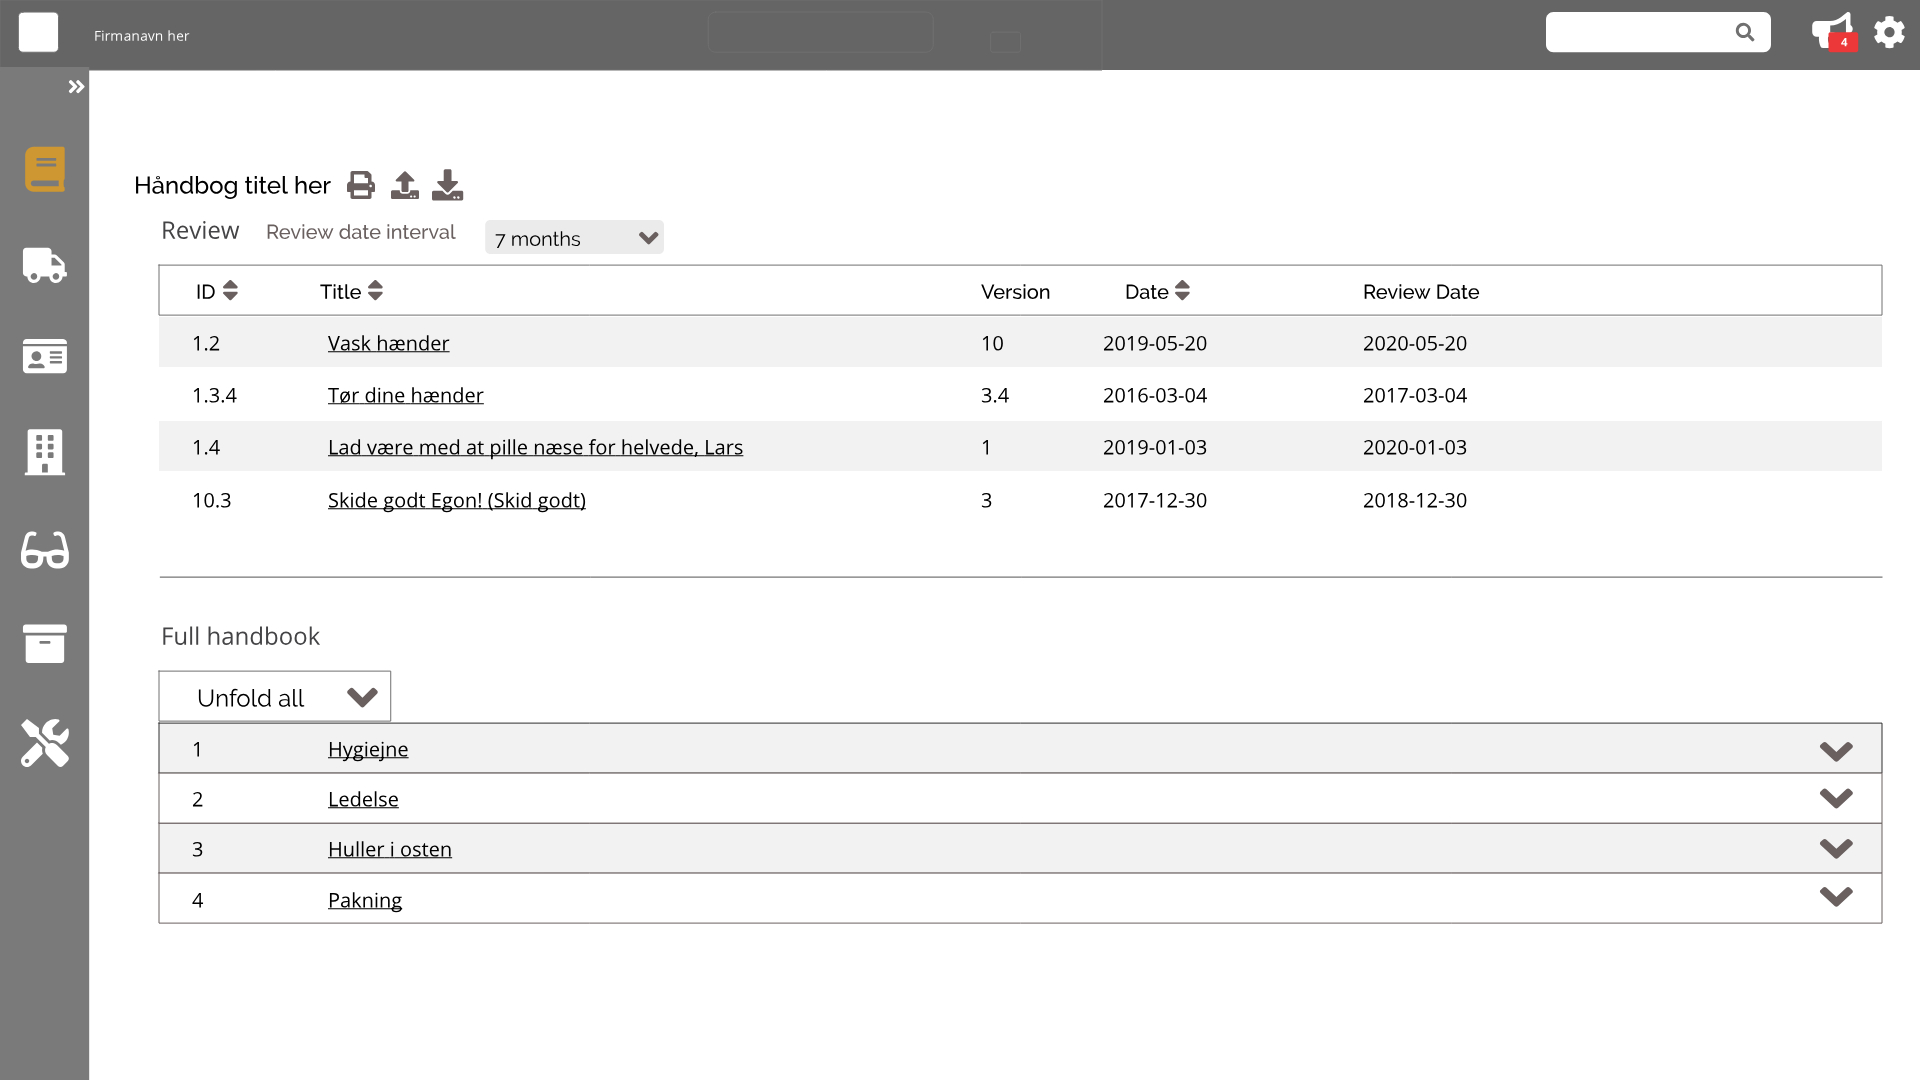
\includegraphics[width=0.7\textwidth]{billeder/ForsideFoldedSidebar.jpg}
		%\label{fig:3-main}
	\caption{Mockup interface of folded sidebar with icons}\label{fig:mockupSidebarIcon}
\end{figure}

The last implementation of the application could continue to prepare for the last usability test of type validation test. 

\subsection{Fourth usability test}\label{fourthtest}
The fourth usability test was conducted on Ipsen, Ipsen's husband and their daughter. 
The reader, writer and administrator roll were all been tested in the application. 

\subsubsection*{Purpose and objectives of the fourth test}
The usability issues from the first test has been corrected and ready to be tested to determine whether the new functionalities are improved or not. 
All the rolls need to be tested as well as the recently added functionality which are required by the system definition. 
The department and user management in the application will also be a part of the testing. The task list for the fourth usability test can be found in \Cref{sec:utest4tasklist}.
The use cases that will be tested are listed below.

\begin{itemize}
	\item Access current handbook (exclude the first time login)
	\item Add new file to the system
	\item Approval new version or document
	\item Access archive 
	\item Add user 
	\item Edit user information
	\item Manage user 
	\item View who has read a document 
	\item Manage departments
\end{itemize}

The functions that will be tested can be seen below.

\begin{itemize}
	\item Add document
	\item Add version
	\item Approve version
	\item Request approval
	\item Update user
	\item Delete user
	\item Add user
	\item Add department
	\item Add user to department
	\item Add document to department
	%\item Download archive 
\end{itemize}

\subsubsection*{Results of the fourth test}
The detected usability issues are present and categorize in table 
\Cref{tab:utest4} which will be clarified afterwards. 

\begin{table}[H]
	\begin{center}
	\begin{tabular}{| c | m{15em} | c | c | c | c | c | c |}
		\hline
		\# & \textbf{Identified usability issues} & Role & Critical & Serious & Cosmetic \\
		\hline
		 1 & The notification button are not visible & All & & & x \\
		\hline
		 2 & Confusion concerning the working file & A, W & x & & \\
		\hline
		 3 & Confusion how to add more than one approver & A, W & x & & \\
		\hline
		4 & No document ID when adding associate documents to a department & A & & & x\\
		\hline
		5 &  Confusion about upload and download button & A, W & x &  &\\
		\hline
		6 & No approve button on awaiting approval document's view & A, W &  & & x\\
		\hline
		7 & No cancel button when edit department & A & & & x\\
		\hline
		8 & Deleted user should not appear while edit department & A & & & x \\
		\hline
		9 & Edit department user list present username & A &  & & x \\
		\hline
		10 & The cursor needs be a pointer when hovering over a row & A &  &  & x \\
		\hline
		11 & When deleting a user the dialog box  does not specificity which user & A & & & x\\
		\hline
		12 & No indication of the who are currently logged in & All & & & x \\
		\hline
		13 & No indication that the awaiting approval had been approved by you & A, W & & x & \\
		\hline
		14 & Both name and username was edited & A & & x & \\
		\hline
	\end{tabular}
	\end{center}
	 {\raggedright Notes. A denotes for administrator role, W denotes for writer role and R denotes for reader role.\par}
	\caption{Identified issues for the fourth usability test}\label{tab:utest4}
\end{table}

The preparation for the second usability test was not done thoroughly because of the time pressure and poor planning. 
The documents in handbook that test subject need to find according to the  described task list were not the same in the application. 
The application had not been tested thoroughly to check whether the test subject would be able to complete the tasks.
Therefore lots of error did appeared during the tests.  
%Det med at beder bruger om at rette i en fil uden for system er forvirrende så det skal man undgå og bare beder dem at upload en dummy fil 

The identified issue '1' occurred when Ipsen was asked to find the notification button. However, there was no notification alert as the notification functionalities was not complete at this point. 
Ipsen commented that the notification button was quite invisible as the notification icon had the almost the same color as the top bar.
%hedder det topbar? 

The identified issue '2' appeared when Ipsen was asked to upload a new version to the handbook. 
New functionality had been added which was the option to both upload pdf file and working file (excel, word etc.), see \Cref{fig:WorkingFile}
Administrator or writer would be able to download working file and easily edit the file. 
Ipsen did not understood what was meant by upload a working file and its purpose.
% Ipsen's husband on the hand understood how the working file worked. 
% Since the application are developed to Ipsen this issue will be categorized as critical. 
A conclusion had been reached to only upload pdf file for simplicity's sake. 
Since administrator would usually store all the working files on the pc. 
And typically the document would be printed out to write directly on it therefore there is no need to upload a working file. 

\begin{figure}[H]
	\centering
		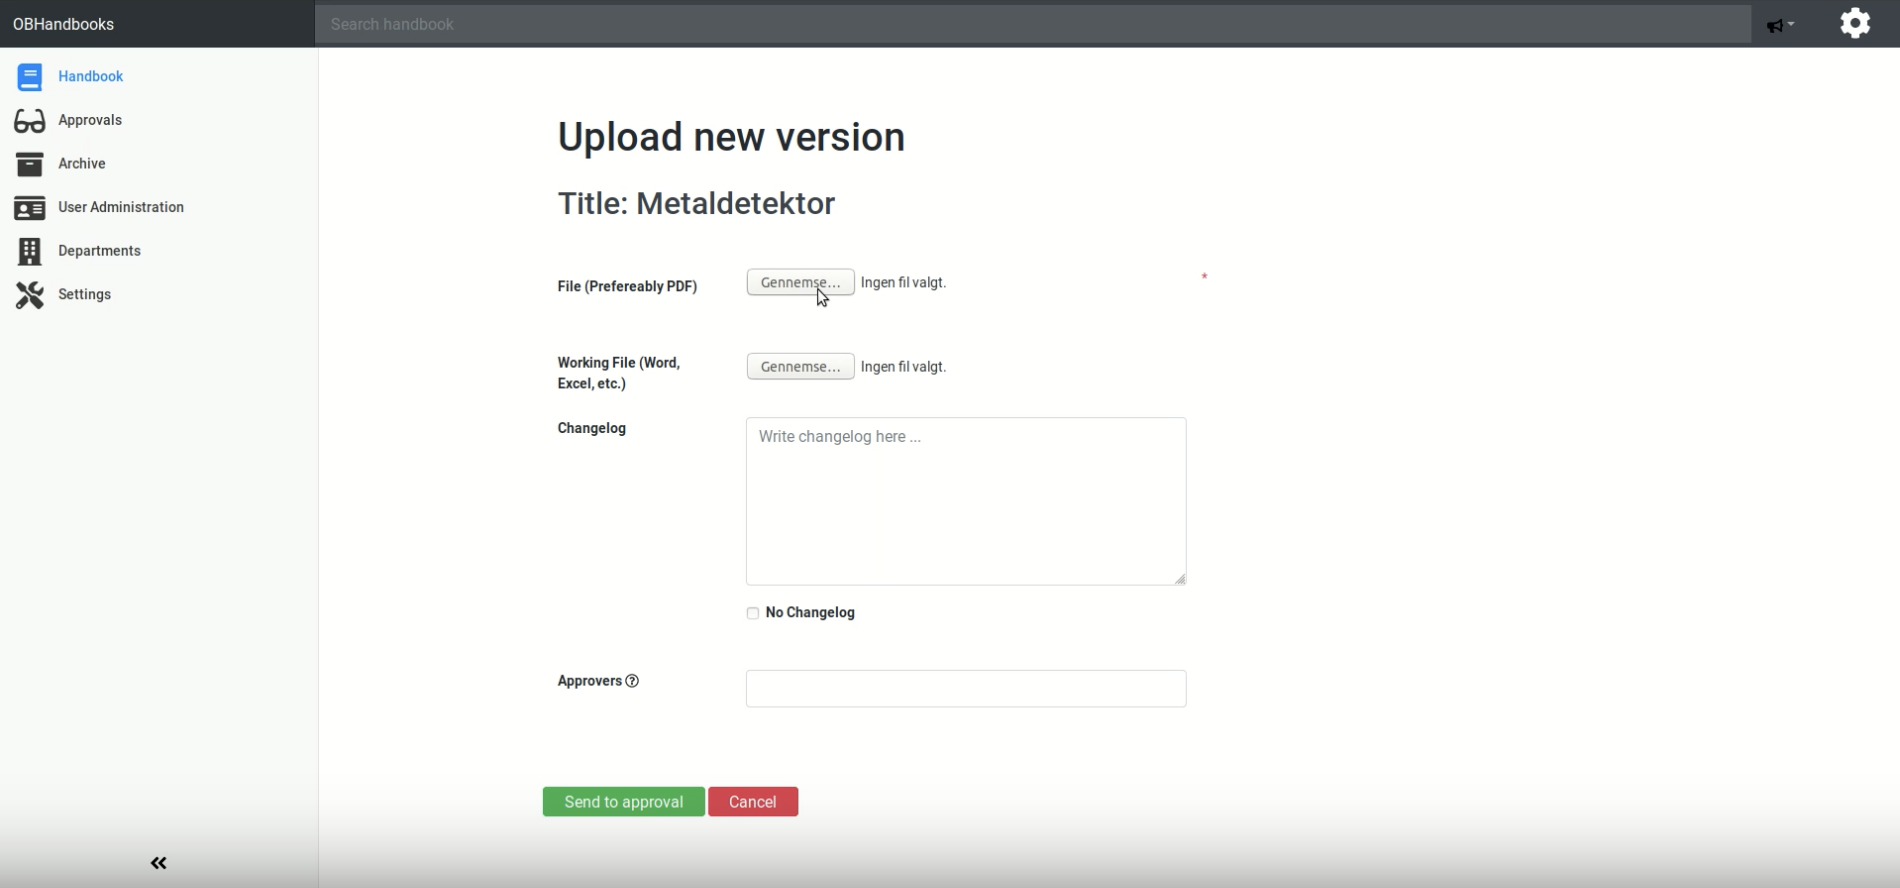
\includegraphics[width=0.7\textwidth]{billeder/WorkingFile.png}
		%\label{fig:3-main}
	\caption{Upload new version page with working file option}\label{fig:WorkingFile}
\end{figure}

The identified issue '3' discovered when there was confusion of how to add multiple approvers while uploading a new version.
To solve this issue a guide text will be added. 

The identified issue '4' noticed while adding documents to a department and document ID was missing. 
Both document ID and name needed to be listed.

The identified issue '5' occurred when asking to upload a new version to a document. 
The upload and download icons were not intuitive enough on their own on the main page and they also looked similar, see \Cref{fig:MainInterfaceAdmin}. 
Ipsen preferred a button with text instead as no doubts would appear. 
Ipsen also mentioned how the upload icon on the main interface would not reflect the right mindset in the workflow. 
An "Add" icon would be more suitable where afterwards user would be able to press on an "upload" icon. 

\begin{figure}[H]
	\centering
		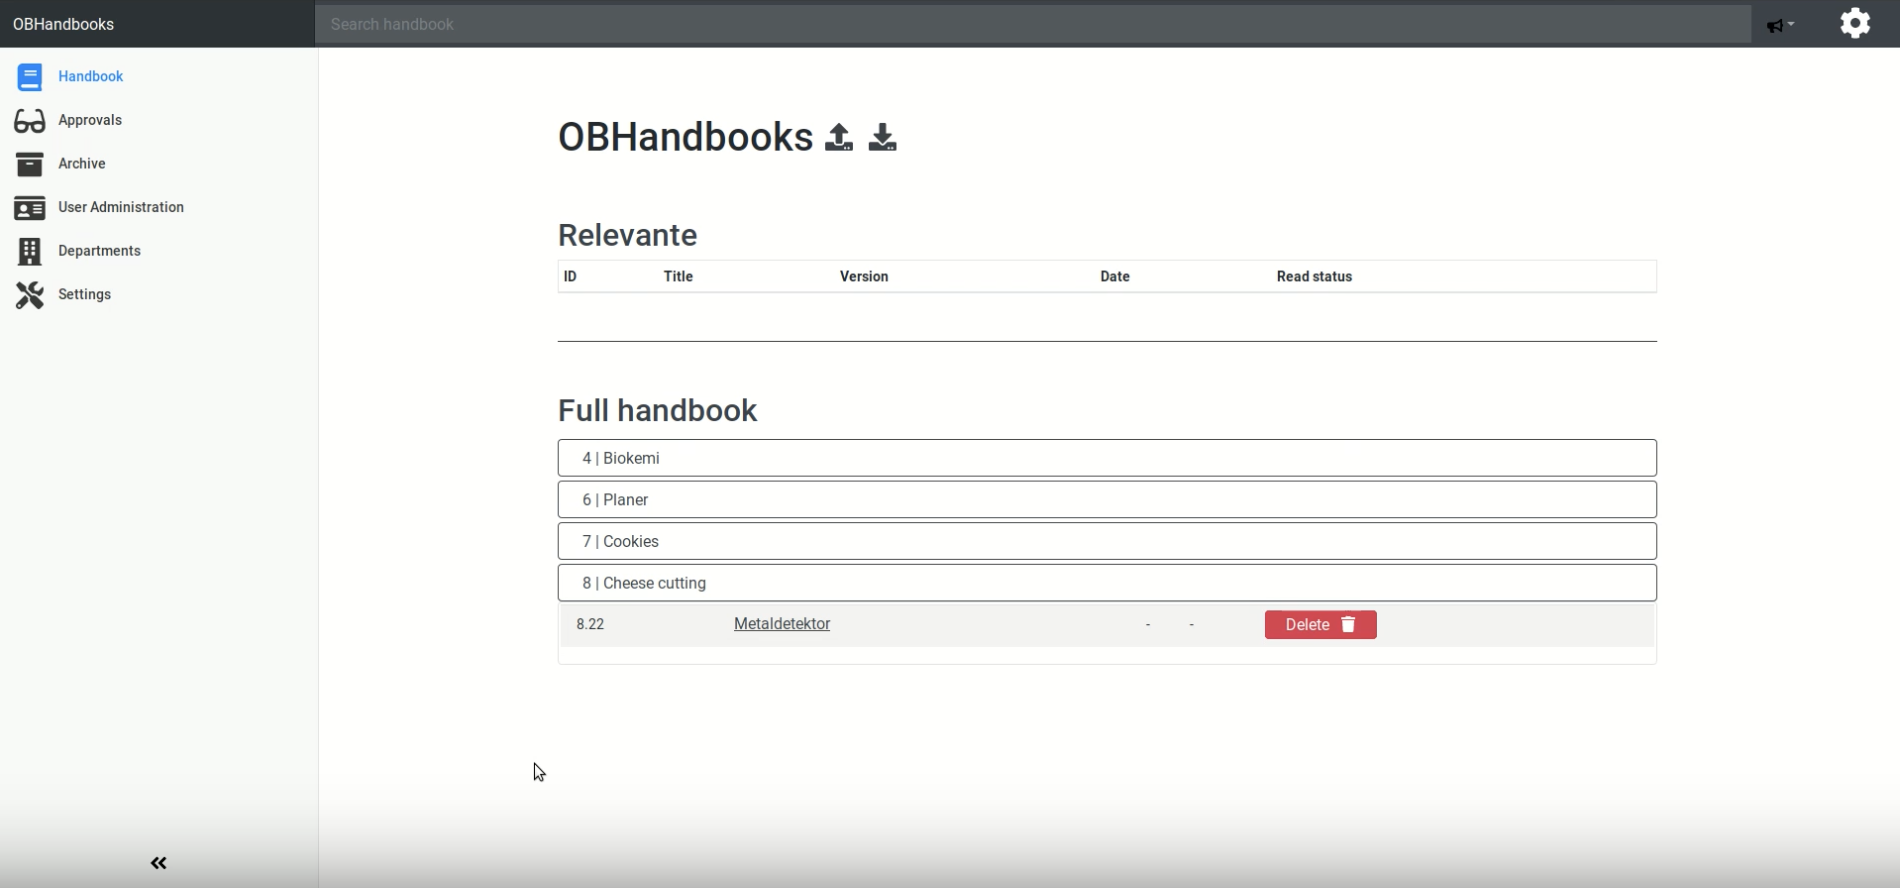
\includegraphics[width=0.7\textwidth]{billeder/MainInterfaceAdmin.png}
		%\label{fig:3-main}
	\caption{Main interface for admin role}\label{fig:MainInterfaceAdmin}
\end{figure}

The identified issue '6' was discovered when Ipsen needed to approve an approval request.  
When entering the document view a approve button should also appear so administrator did not need to go back to the previous page to press the approve button. 

The identified issue '7' was noticed when adding user and document to a department where no cancel button appear. 

The identified issue '8' occurred when adding user and document to a department and deleted user still presented in the list as long random character and number combination. The identified issue '9' was also discovered that user represented as username and not name. 

The identified issue '10'  and '11' was discovered when deleting a user.
Error such as accidently deleting a unintended user could most likely occur.  
Ways to indicate and make it clear are as follow; the user row the cursor is hovering over will be highlighted or dialog box needs to specify which specific user will be deleted.  

The identified issue '12' occurred when Ipsen's husband mentioned that it would be helpful if the interface showed which user that was currently logged in the application. 

The identified issue '13' was discovered once administrator had approved an awaiting approval request that still need to be approved by others. 
No indication was showed that it already had been reviewed and approved.
The user must therefore remember which document they had approved. 

The identified issue '14' occurred when administrator was asked to modify the a user's name. 
Administrator was able to both edit a user's name and username. 
It turned out both name and username was edited. 
% Ved ikke hvad der skal skrives her ift. at admin ikke burde have lov til at ændre i username?

% Confusion regarding upload a new version whether to find the file in the application or the system  -
% Når filen ikke er en pdf fil burde man kunne download filen fordi det vises ikke i preview. men det problem fjerner vi hvis det kun er pdf filer der må uploades?

During the debriefing session Ipsen was asked if there was other functionality she desired that the application provide?
She mentioned that she wished to be able to access a list of departments a user was associated to and a list of all the documents the user did not read. 
Administrator could make a mistake and added the user to a wrong department for that reason. 
Ipsen suggested that if a user did not read an associated document over a week department head would be alerted.
If a user still not had read by over two weeks administrator would be alerted. 

It had also come to the conclusion that the department head should be the one who keeping track and ensure that the employee had read the associated documents. 
Therefore the department heads belongs to a writer role with access to read status. 

Furthermore, Ipsen had hoped that the application would be able to change the date and the version in the actual document header. 
However, the application does keeps track of the date and the version but readers also need to know whether they stand with the valid version in printed form. 
%Ipsen ønsker at systemet også kan ændre side hoved i selve fil/dokumentet , hvor der står udgave og dato på - når man printe det ud, så kan man se at det er den opdateret version de har der. Forslag: ku man når man upload dokumentet at du i virkelighed send et blank header med pdf format og så bliver det udfyld og også i håndbogen? i dont get that

The writer rights regarding if a writer are allowed to archive a document in the handbook had also been clarified. 
Ipsen pointed out that only administrator are able to archive documents. 

In the end of the debriefing session activating account for the first time login and its process was represented to Ipsen instead of testing it as a part of the usability test. 
% Ved ikke om det burde nævnes? 


% Perspektiveret: bliver enige om at når man laver en %department at man markerer en bruger en som department %heads og det er dem som får notifikationer.
% approval id er ikke dok ide?

%%% Positive kommentarer  %%%
%Ændre brugernavn var ligetil
%Ipsen kunne finde changelog nemt.
%Department var meget nemt at forstå

%Der mangler en unfold all dok under full handbook- vi har ikke unfold all chapters?

%Tove
%Lægger mærke til at layout og farven ikke er det samme som de andre pc?
%Problemer med at opret en ny dok
%Archive ser mærkelig ud?

%Udført på den forkerte version af programmet

%\subsection{Usability issue that are not a bug}

% brugervenlighed issues som ikke er bug, kan ikke hvad der blev snakket om